%
% Network Topologies
%

\section{Network topologies} \index{Network topologies}\label{sec:network_topologies}

\dropcap{A}{s} quantum (or classical) networks inherently reside on graphs, it is important to introduce some of the key graph structures of relevance to networking and some of their properties of relevance to quantum networking protocols.

In principle a network could be characterised by any connected graph whatsoever. However, there are certain structures and patterns that emerge very frequently and deserve special attention.

It is paramount that QTCP protocols have the capacity to deal with the diverse network topologies that are likely to present themselves in the future real-world quantum internet. Some of the graph-theoretic algorithms that we rely on in our QTCP protocol (Sec.~\ref{sec:graph_theory}) are computationally efficient for \textit{arbitrary} graph topologies, even more so for certain classes of graphs exhibiting particular structure, such as tree graphs or complete graphs. Others, however, are computationally inefficient in general, but may have efficient approximation algorithms for some or all classes of topologies.

We will now review some of the graph structures most likely to arise in quantum networks, learning from the structures that have become ubiquitous in classical networking.

%
% Point-To-Point
%

\subsection{Point-to-point} \index{Point-to-point topologies}

The most trivial network topology, which also acts as the elementary primitive from which our other topologies will be constructed is a simple dedicated point-to-point (P2P) connection between two parties, where the sender and recipient of a packet reside on neighbouring nodes.

Such P2P connections may be reserved exclusively for the two connected neighbouring nodes. In this instance, the packets' \textsc{Routing Queue}s trivially specify just the recipient. Alternately, the P2P link may be an intermediate step between more distant sender/recipient pairs.

In the case whereby the P2P connection is reserved exclusively for a particular sender/recipient pair, the link has the property that there is no competition between multiple users sharing the channel, and the QTCP stack needn't concern itself with dynamic routing strategies\footnote{Assuming the P2P channel has sufficient capacity to meet demand and exhibits better cost metrics than other potential redundant, indirect routes.}. This significantly simplifies network scheduling algorithms (Sec.~\ref{sec:strategies}), and a \textsc{First-Come First-Served} (i.e chronologically ordered FIFO queue) strategy may be employed. Furthermore, packet collisions cannot occur, thereby improving network efficiency.

In the case whereby the P2P connection is not reserved for exclusive use between a single sender/recipient pair, but shared between different competing routes in the network, the importance of network routing strategies manifests itself. Now competition for access to the channel will reduce network efficiency, scaling inversely against the number of network participants, and the priorities and costs of packets must be tallied for the purpose of implementing routing strategies.

%
% Complete
%

\subsection{Complete} \index{Complete topologies}

The complete graph, denoted $K_{|V|}$, is a $|V|$-vertex graph where every vertex has an undirected link to every other. From a networking point of view, this can be regarded as the extremity of exclusive-use P2P networking, whereby every node has a direct link with every other. Thus, any sender can directly communicate with any receiver, via a dedicated direct channel, with no need to utilise any indirect routes. This topology has the favourable property that although any node can communicate with any other, by exclusively utilising direct P2P links we achieve several benefits:
\begin{itemize}
\item Packet collisions can be mitigated entirely, thereby maximising network efficiency.
\item Competition for the use of links can be eliminated, minimising congestion and the need for buffering (i.e quantum memory).
\item Network costs can typically be minimised, as every route only traverses a single link, and there will be no accumulation of costs.
\item The network has maximal route redundancy, making it the most tolerant against link failures\footnote{To disconnect a given node from the network, all \mbox{$|V|-1$} links emanating from it must be broken, otherwise redundant routes to the remainder of the network will exist.}.
\item A trivial \textsc{First-Come First-Served} routing strategy can be employed, eliminating the need for any dynamic or computationally complex strategies.
\item If the network allows indirect routes to be established, the maximal redundancy of the topology also maximises the ability for routing strategies to engage in load-balancing across routes.
\item In the special case of a symmetric complete graph, whereby all edge weights are approximately equal, the shortest path between any two nodes is trivially the P2P link between them, and no complex scheduling algorithms are required.
\end{itemize}
However, these highly desirable benefits come at the expense of requiring the most elaborate and expensive network, with maximal interconnectedness.

This type of topology could arise in, for example, international-scale networks, where links of very high bandwidth (and value) between nations or continents need to be maximally utilised, which would be undermined by sparse, shared network topologies. Additionally, in this instance route redundancy will be highly valued, as the isolation of one continent from another would be catastrophic to the functioning of the global network.

Fig.~\ref{fig:complete_graph} illustrates the $K_{15}$ graph. The number of edges scales as $O(n^2)$. Clearly route-finding is trivial, since there is always a direct link from sender to receiver, with no possibility of collisions with other packets, requiring $O(1)$ search time (assuming all users are communicating only via their direct links with one another, which may not strictly be the case when costs are factored into strategies).

\begin{figure}[!htb]
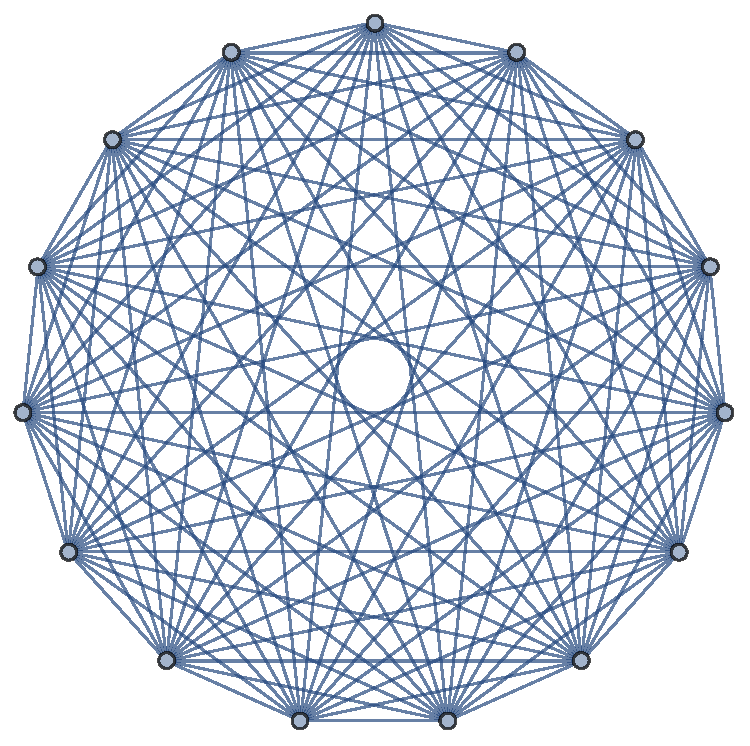
\includegraphics[width=0.35\textwidth]{K_15}
\caption{The 15-vertex complete graph, $K_{15}$. Every vertex has an edge to every other, with a total of 105 edges.} \label{fig:complete_graph}
\end{figure}

%
% Lattice
%

\subsection{Lattice} \index{Lattice topologies}

A lattice graph is simply an \mbox{$n\times m$} lattice of vertices (of any geometry, e.g squares), connecting each vertex to its immediate geometric neighbours. This type of graph is useful when link costs are measured in terms of Euclidean distances, and nodes have nearest neighbour links. An example is shown in Fig.~\ref{fig:lattice}.

\begin{figure}[!htb]
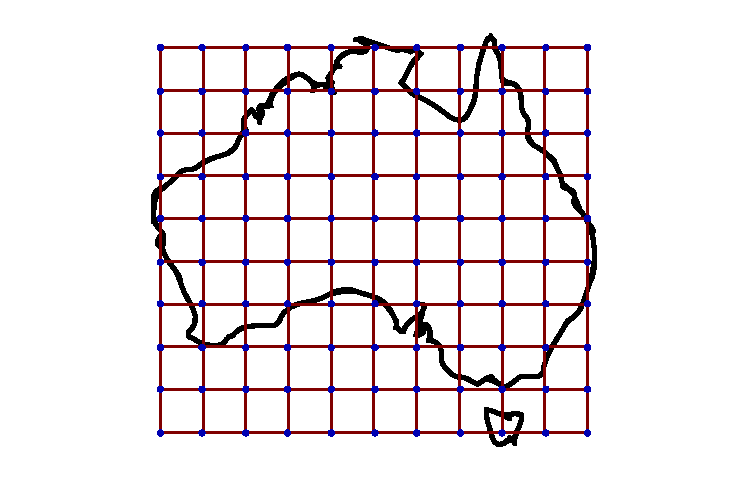
\includegraphics[width=0.35\textwidth]{lattice}
\caption{A \mbox{$10\times 11$} square lattice graph, and how it might represent a network topology with geographically associated costs. Notice that Hobart has no internet connection (why even include Tasmania at all?).} \label{fig:lattice}
\end{figure}

A slightly distorted lattice graph, in which vertices have been dragged around geometrically to match, for example, cities within a country, closely resembles the topology of the network. Similarly, if the nodes represent houses in the street layout of a highly regular city like Manhattan, a lattice may be a good approximation.

In the case of a balanced lattice, in which all edges are of equal weight, the cost of a route is the sum of the number of steps in the vertical and horizontal directions, also known as the Manhattan or $L_1$ distance,
\begin{align}
L_1 = |x_\mathrm{start} - x_\mathrm{finish}| + |y_\mathrm{start} - y_\mathrm{finish}|.
\end{align}
In this case, route finding is simplified, since \textit{all} routes, which strictly traverse in one direction vertically and one direction horizontally, are optimal and of equal distance.

%
% Tree
%

\subsection{Tree} \label{sec:tree_graph} \index{Tree topologies}

A tree is a graph containing no cycles, only \textit{branches}. There are many uses for tree graphs, but one property is of particular convenience in many applications: because the graph is acyclic, there is always exactly one path from any vertex to any other. This mitigates the need for shortest-path algorithms designed for general graphs, and simplifies route-finding algorithms (to be discussed in Sec.~\ref{sec:path_exp}). However, this brings with it the drawback that the topology is most vulnerable to link failures, since the removal of any link from the tree will separate it into a bipartite graph, making communication between the two disjoint subgraphs (which are also trees) impossible, as there are no redundant routes. In a sense, tree graphs can be considered the polar opposites of complete graphs.

Trees are specified entirely by \textit{branching parameters} ($b_i$) -- the number of child nodes emanating from a given node, $i$. In general, branching parameters may be distinct for each node, although often trees with symmetries in their branching structures are considered, such as the balanced trees discussed in Sec.~\ref{sec:bal_tree}. A node terminates a branch if its branching parameter is zero (i.e it has no children).

The \textit{depth} ($d$) of a tree is the maximum number of steps from the root node to a terminating node with no children. The depth scales between \mbox{$d=O(|V|)$}, for the trivial linear tree (\mbox{$b_i=1$}), and \mbox{$d=O(\mathrm{log}|V|)$} for non-trivial branching parameters (i.e \mbox{$b_i\neq 1$}).

The worst-case number of edges that must be traversed to reach any vertex from any other is $2d$, which implies that accumulated cost metrics scale as at most \mbox{$c=O(|V|)$}. Trees are the most frugal graphs in their number of edges, which are fixed at \mbox{$|E|=|V|-1$}, irrespective of the branching parameters, since because the graph is strictly acyclic, every addition of an edge requires the addition of exactly a single vertex. This makes tree graphs the cheapest to construct in terms of physical resource usage.

%
% Balanced Tree
%

\subsubsection{Balanced tree} \label{sec:bal_tree} \index{Balanced tree topologies}

A balanced tree is a tree with a regular, self-similar structure, in which every node at a given depth is the parent of the same number of sub-nodes, all separated by the same edge weights. That is, the network has a hierarchical structure, subdividing into identically structured subnetworks. Such a network is characterised by just two parameters -- the branching parameter, $b$, and the depth, $d$. Some examples of balanced trees with different $b$ and $d$ are shown in Fig.~\ref{fig:tree_example}.

\begin{figure*}[!htb]
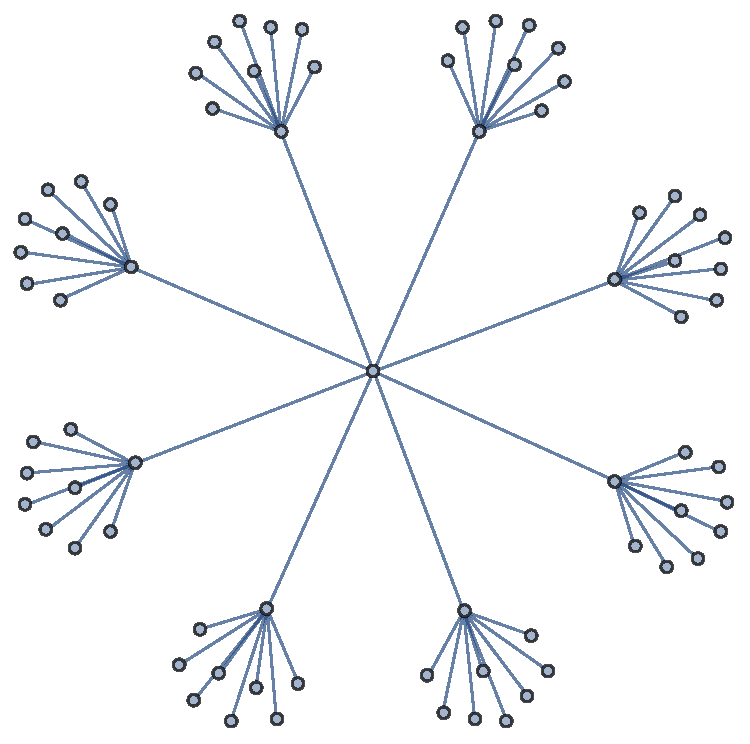
\includegraphics[width=0.325\textwidth]{tree_3_8}
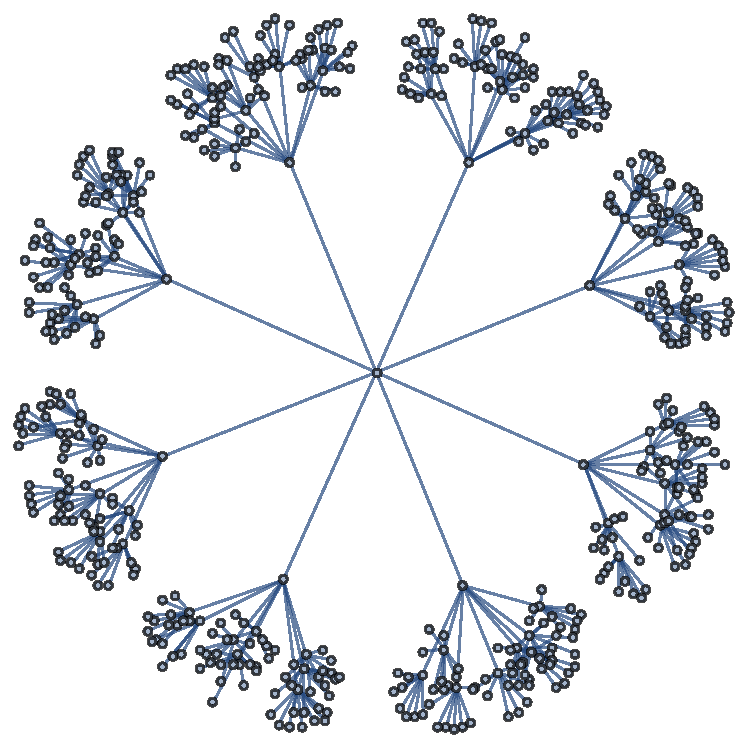
\includegraphics[width=0.325\textwidth]{tree_4_8}
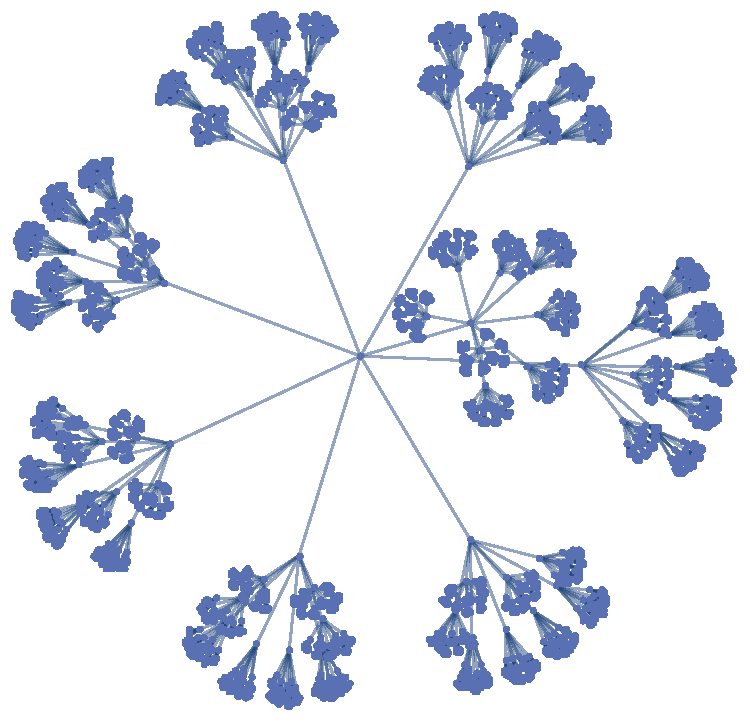
\includegraphics[width=0.325\textwidth]{tree_5_8}
\caption{Balanced tree graphs with branching factor $b=8$, and depths $d=3,4,5$. Despite having no redundant paths, the hierarchical structure of balanced trees somewhat resembles that of real-world networks, which are typically decomposed into a pyramid scheme of progressively smaller subnetworks.} \label{fig:tree_example}
\end{figure*}

This type of structure is (approximately) natural in many realistic scenarios. Consider for example a network containing a hierarchy of clusters of nodes representing a LAN, followed by a neighbouring internet router, followed by a city-wide router, followed by a country-wide router. In such a case, this type of general structure is typical (although more realistically one might expect the branching parameter to vary with depth).

A special case is when \mbox{$d=1$}, which we refer to as a \textit{star} graph. This might arise naturally when a series of subnets are connected together via a central router (e.g Fig.~\ref{fig:net_hierarchy}), with no further hierarchy in the network.

%
% Random Tree
%

\subsubsection{Random tree} \index{Random tree topologies}

While balanced trees accurately capture the hierarchical nature of realistic networks, they are somewhat contrived in their perfect symmetry. The subnetworks in a given network are not likely to actually all be identical. Random trees are perhaps more realistic, in that their tree structure captures the hierarchical nature of real-world networks, and also their highly ad hoc nature.

To construct a random tree we simply randomly choose a branching parameter, according to some arbitrary distribution, for every node. When a node has \mbox{$b_i=0$}, it terminates the lineage. Some examples of random trees are shown in Fig.~\ref{fig:random_tree}.

\begin{figure*}[!htb]
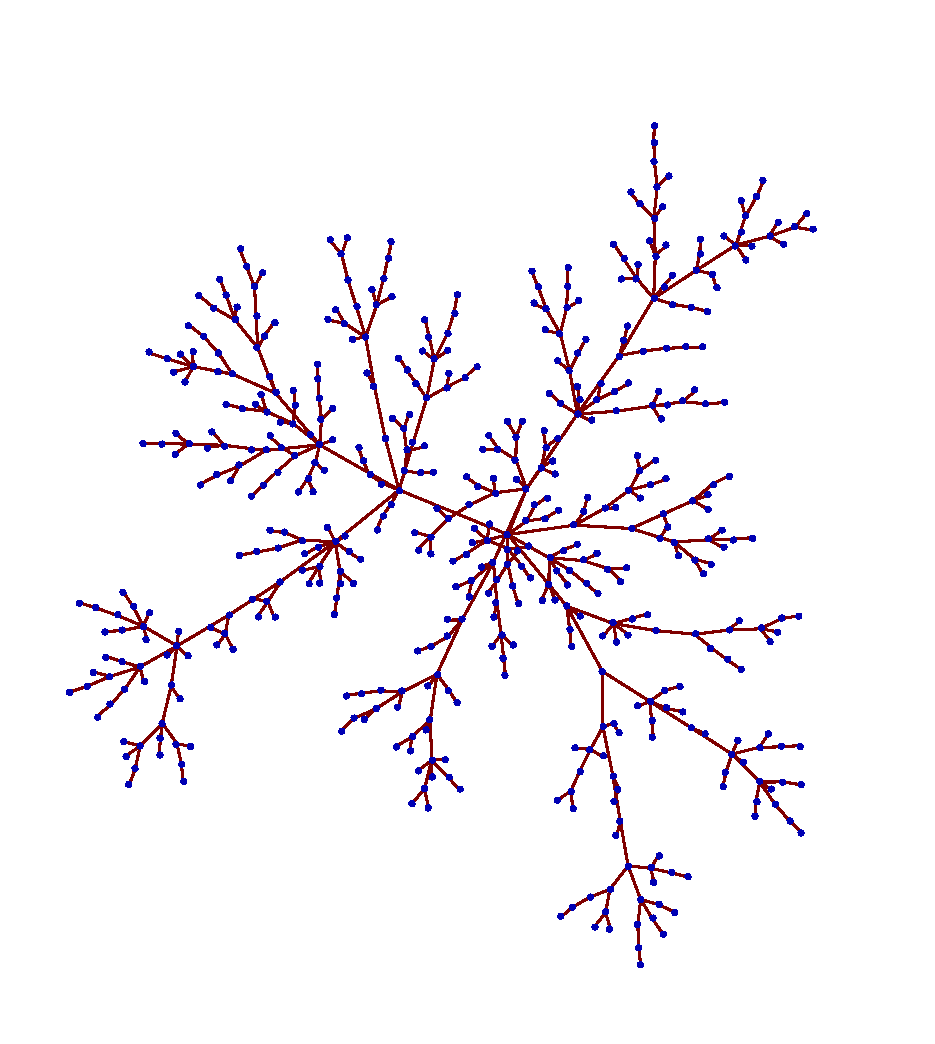
\includegraphics[width=0.47\textwidth]{random_tree_1}
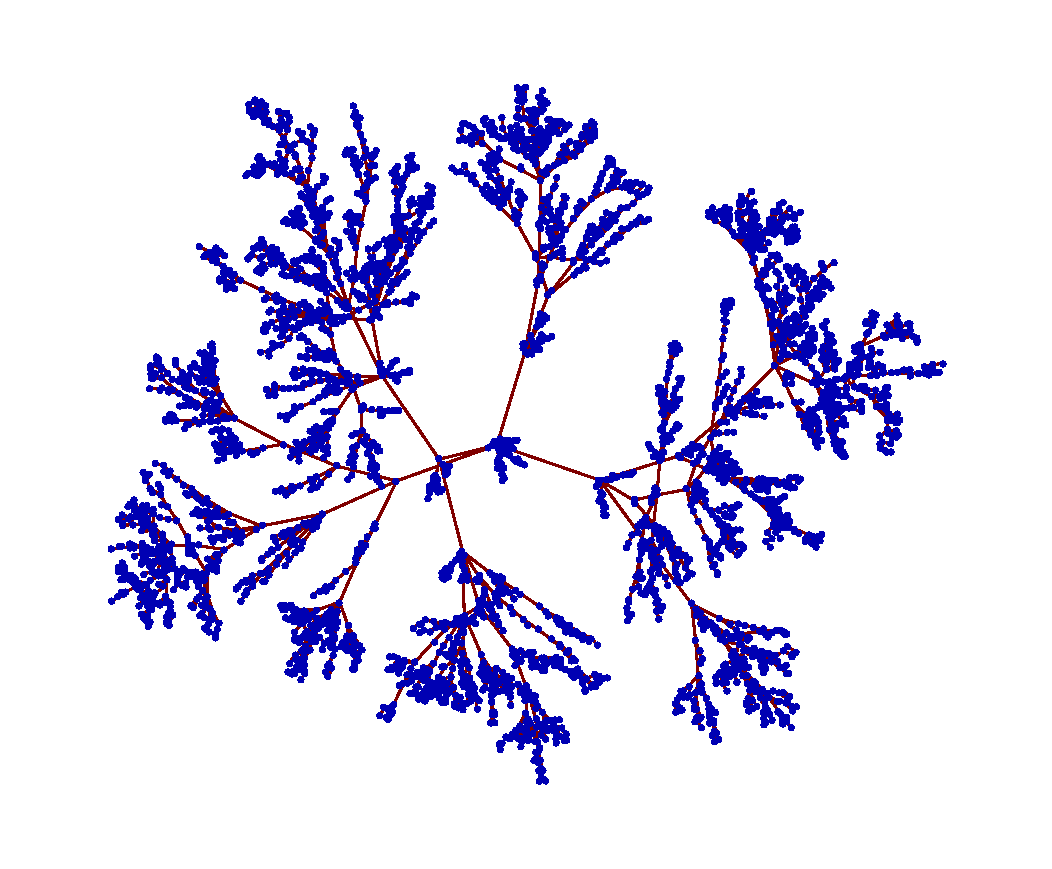
\includegraphics[width=0.47\textwidth]{random_tree_2}
\caption{Random trees with different randomised branching parameters (higher $b$ on the right). When a node has zero branches, it terminates the branch. This type of graph topology qualitatively captures the hierarchical, yet ad hoc qualities of many real-world networks, and may act as a useful test model for simulations.} \label{fig:random_tree}
\end{figure*}

%
% Minimum Spanning Tree
%

\subsubsection{Minimum spanning tree} \label{sec:graph_MST} \index{Minimum spanning tree}

A \textit{spanning tree}\index{Spanning tree} $S$, of a graph $G$, is a tree subgraph \mbox{$S\subset G$}, containing every vertex of $G$. The \textit{weight} of a spanning tree is the sum of all its constituent edge weights. Thus, the \textit{minimum spanning tree} (MST) is a spanning tree that minimises net weight. An example is shown in Fig.~\ref{fig:mst}. See Sec.~\ref{sec:min_tree} for a discussion on MST algorithms.

\begin{figure}[!htb]
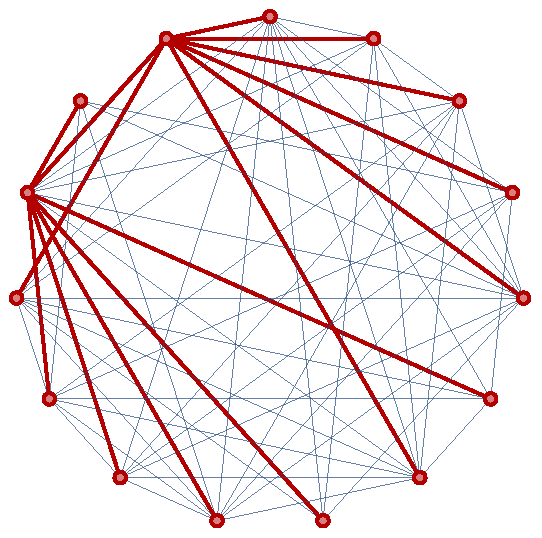
\includegraphics[width=0.4\textwidth]{MST}
\caption{A random graph (blue) with an MST highlighted (red).} \label{fig:mst}
\end{figure}

The calculation of MSTs is most likely to come into consideration when actually performing the initial construction of networks, where we wish to connect all nodes in the network, but using the most frugal possible physical resources. MSTs serve this purpose, and since they are trees, inherit all the same properties of tree networks.

%
% Percolation
%

\subsection{Percolation}\index{Percolation graph}

A variation on any graph, $G$, is to instead have a randomised implementation of it, whereby each of the possible edges \mbox{$e\in E$} or vertices \mbox{$v\in V$} occurs with some probability \mbox{$0\leq p_\mathrm{perc}\leq 1$}. These are referred to as \textit{edge percolation} and \textit{site percolation} graphs respectively.

Adjusting $p_\mathrm{perc}$ allows us to tune between the desired graph (when $p_\mathrm{perc}=1$) and the completely disconnected graph (when $p_\mathrm{perc}=0$). This model is very useful in real-world applications, allowing unreliable channels/nodes to be incorporated into our network model. The analysis of such percolation networks is invaluable for understanding the robustness of such networks to channel and node failures.

%The average number of links emanating from any node is \mbox{$e_\mathrm{av} = (|V|-1)p_\mathrm{edge}$}.

Note that percolation graphs might be disjoint with sufficient defects, in which case the respective network becomes unreliable. Specifically, with sufficiently low $p_\mathrm{perc}$, `islands' may form in the network topology -- small segregated networks, which are unable to interface with the remainder of the network.

For asymptotically large percolation graphs, \textit{percolation theory}\index{Percolation theory} \cite{???} provides thresholds for $p_\mathrm{perc}$ such that routes across the network exist \cite{???}.

Fig.~\ref{fig:perc_graph} illustrates several graphs with different percolation probabilities, and how the larger network segregates into smaller islands as failure rates increase.

\begin{figure*}[!htb]
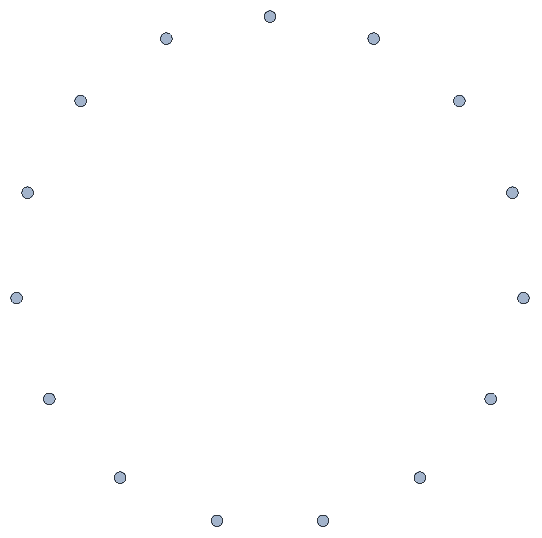
\includegraphics[width=0.325\textwidth]{random_0}
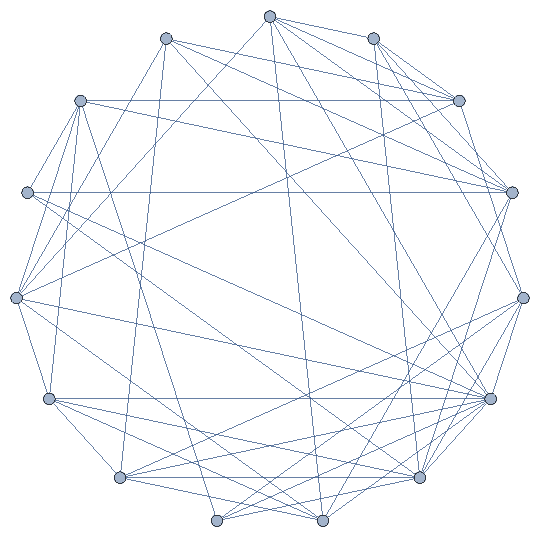
\includegraphics[width=0.325\textwidth]{random_05}
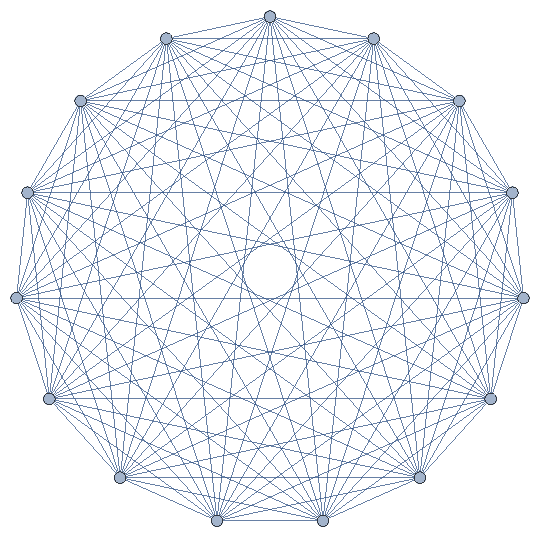
\includegraphics[width=0.325\textwidth]{random_1}\\
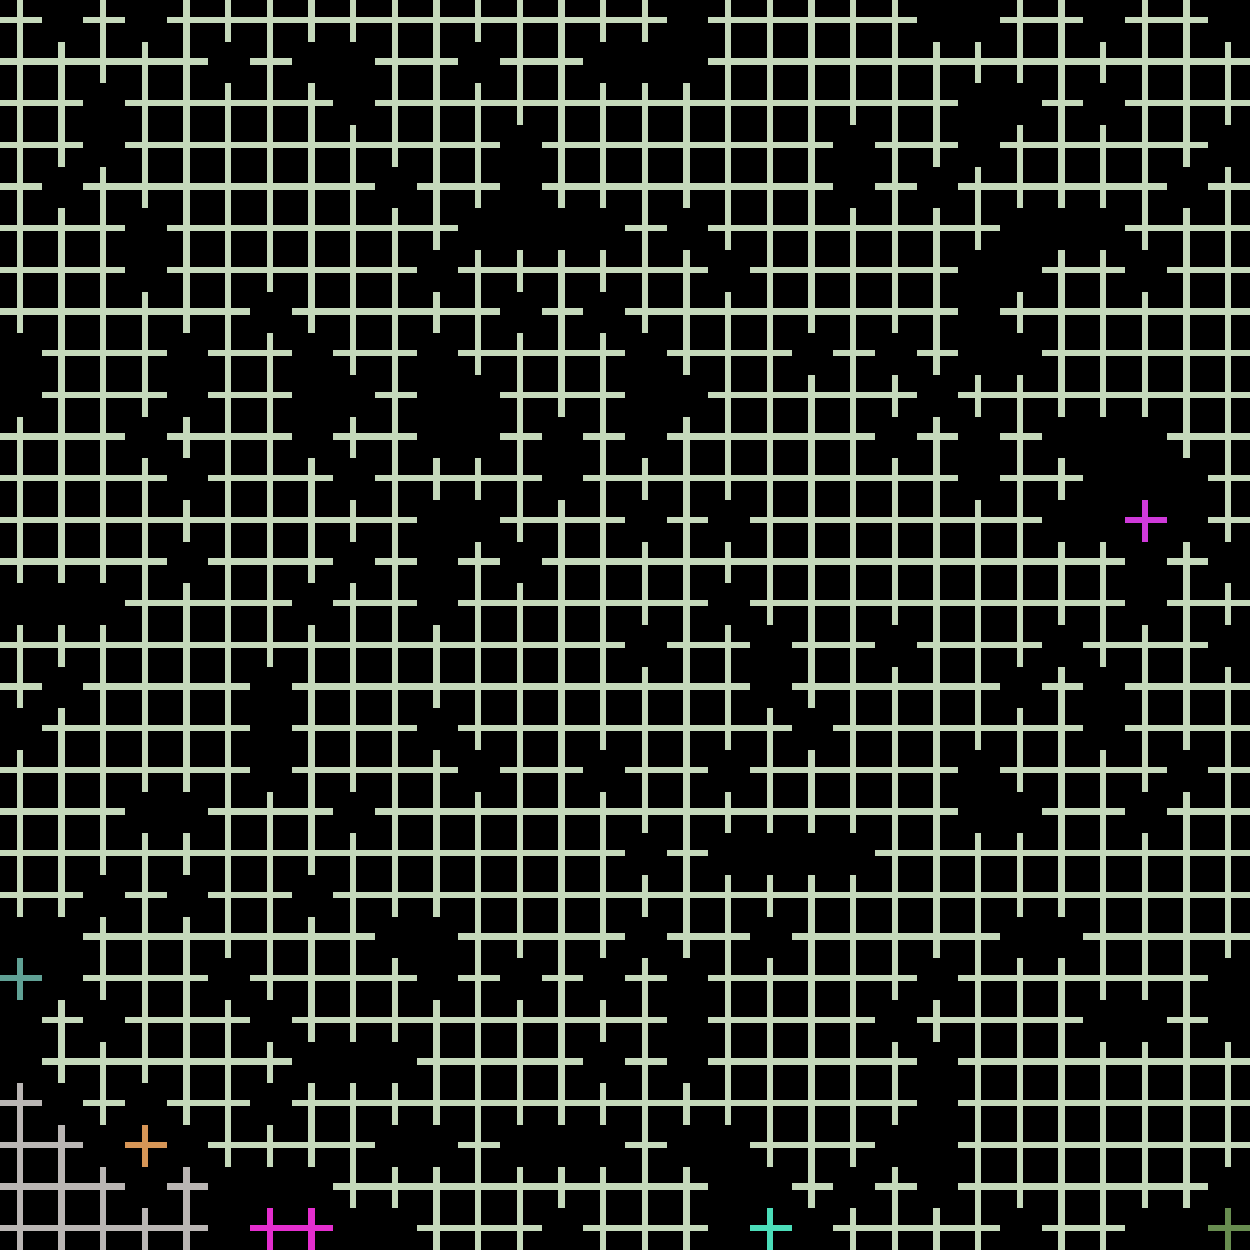
\includegraphics[width=0.325\textwidth]{percolation_1}
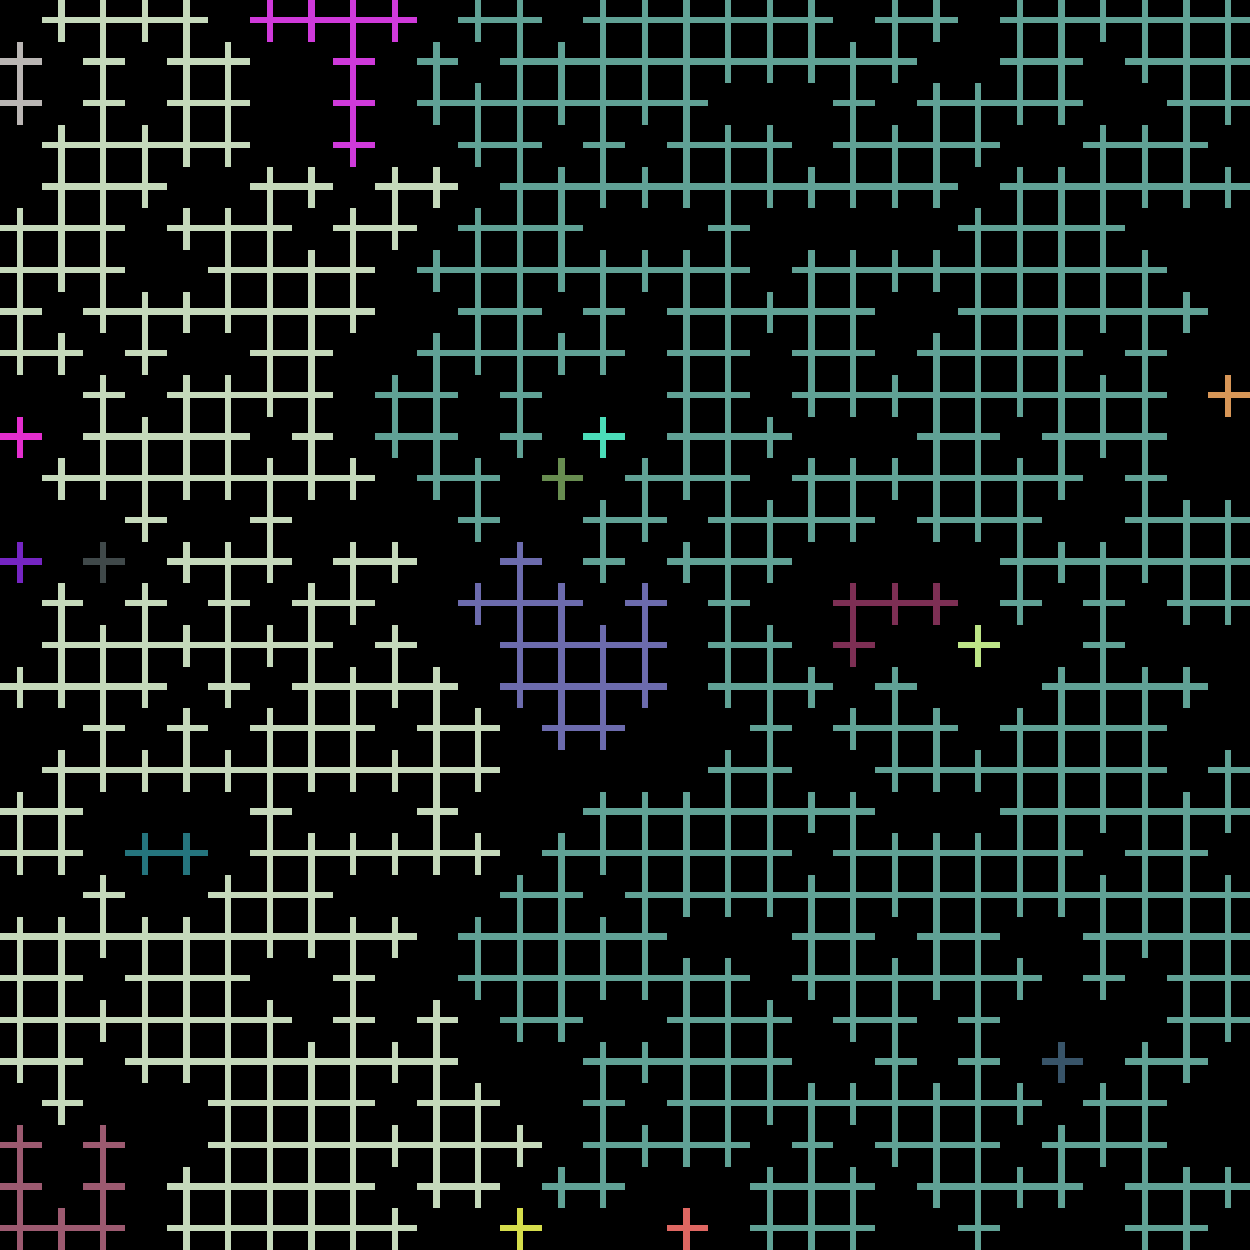
\includegraphics[width=0.325\textwidth]{percolation_2}
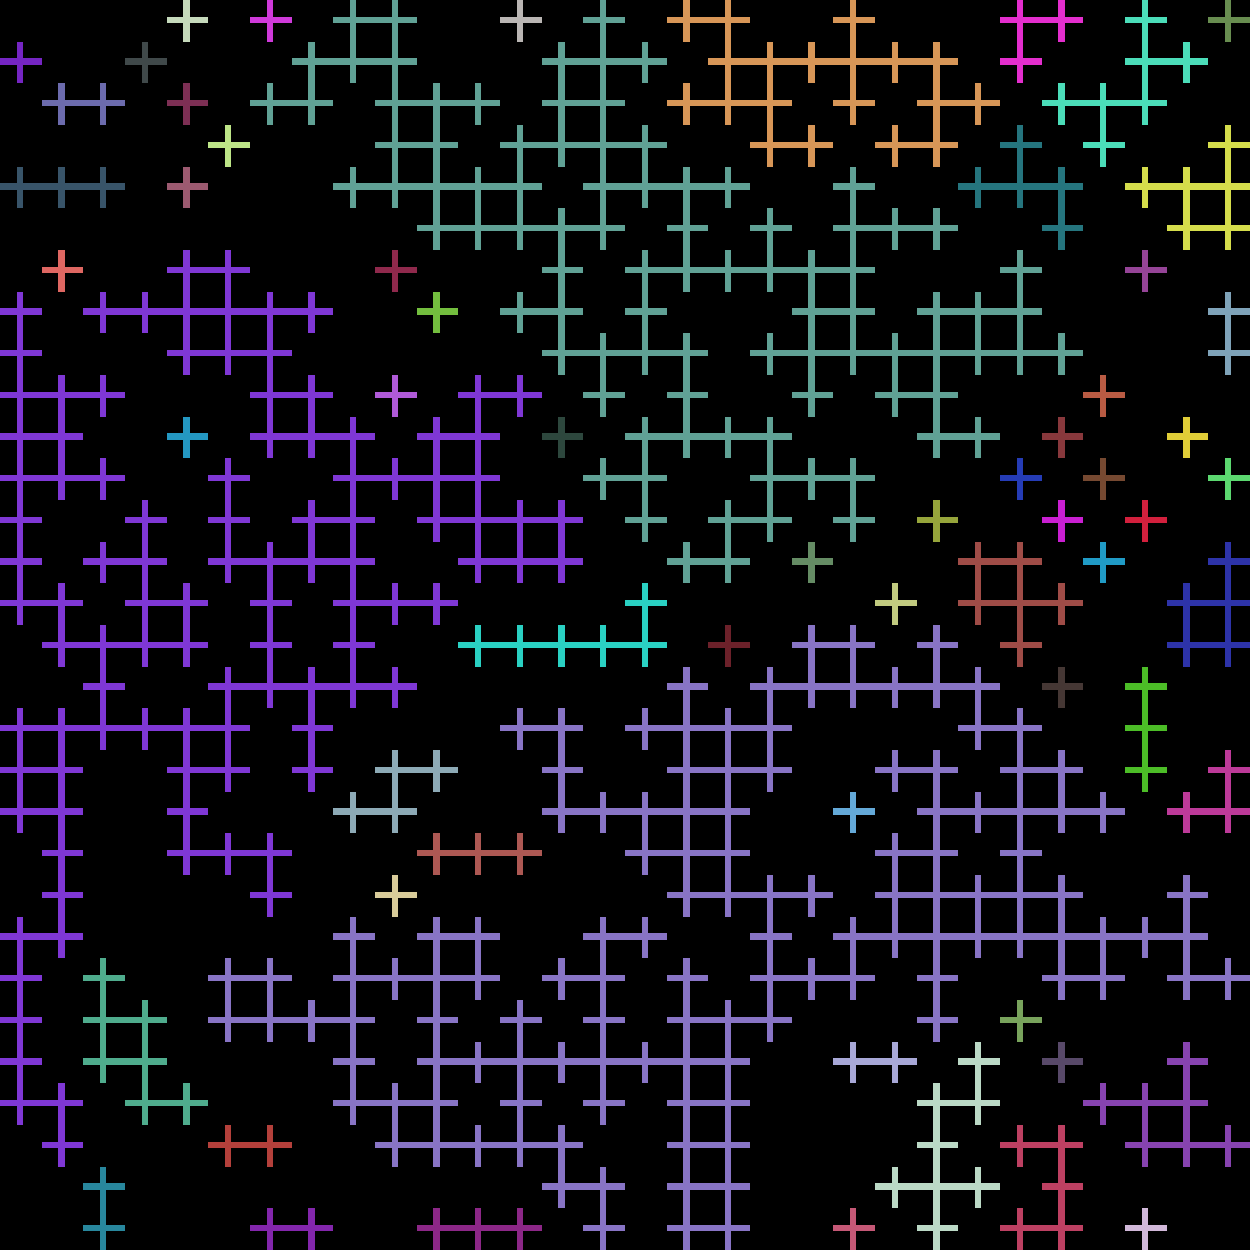
\includegraphics[width=0.325\textwidth]{percolation_3}
\caption{(top) The 15-vertex randomly-connected percolation graph. This is the same as $K_{15}$ in Fig.~\ref{fig:complete_graph}, but where edges are present with probabilities \mbox{$p_\mathrm{edge}=0,0.5,1$} (top to bottom). (bottom) A square lattice graph subject to different percolation rates (node defects). As the failure rate increases, the larger network segregates into smaller disjoint islands (denoted by colour).} \label{fig:perc_graph}
\end{figure*}

%
% Hybrid
%

\subsection{Hybrid} \index{Hybrid topologies}

Real networks are highly unlikely to fit the exact form factor of any of the classes of graphs presented above. Rather, a truly global internet is inevitably going to comprise many subnetworks, each structured completely independently of one another, with little consistency or large-scale planning between them. Who thinks about the broader structure of the global internet when setting up their office network?

For example, at the global scale, it is entirely plausible that the internet might take on a random tree-like structure. But when we get down to a lower level, the tree structure vanishes and is replaced by all manner of different network topologies, run and maintained by different organisations in their own distinct ways.

Furthermore, the real-world internet is not simply a hierarchy of different types of well-known graph structures. Rather, it takes the form of `glued' graphs, whereby networks running over different mediums, or via different operators, each exhibit their own independent graph topologies, meeting at interconnect points that join the different networks. Typically this yields redundancy in the routes between different nodes, ushering in the need for combinatorial optimisation techniques when allocating network resources.

This hybrid network topology is the norm today in our classical internet, and it is entirely foreseeable that a similar trend will emerge in the future quantum internet as quantum technologies become more mainstream, their networking less well structured, and competing, redundant links are in place.

%
% The Internet Web-Graph
%

\subsection{The internet web-graph} \index{Internet web-graph}

Of course, all the topological structures described until now are in-principle constructs. Of most relevance is the \textit{Web-graph}, the graph of the actual internet (or some other real-world network). Fig.~\ref{fig:webgraph} illustrates some example web-graphs. The combination of random, densely and sparsely connected, and tree structures, and its clear hierarchy are all evident. This encourages our intuition of the different types of structures present in realistic networks.

\begin{figure*}[!htb]
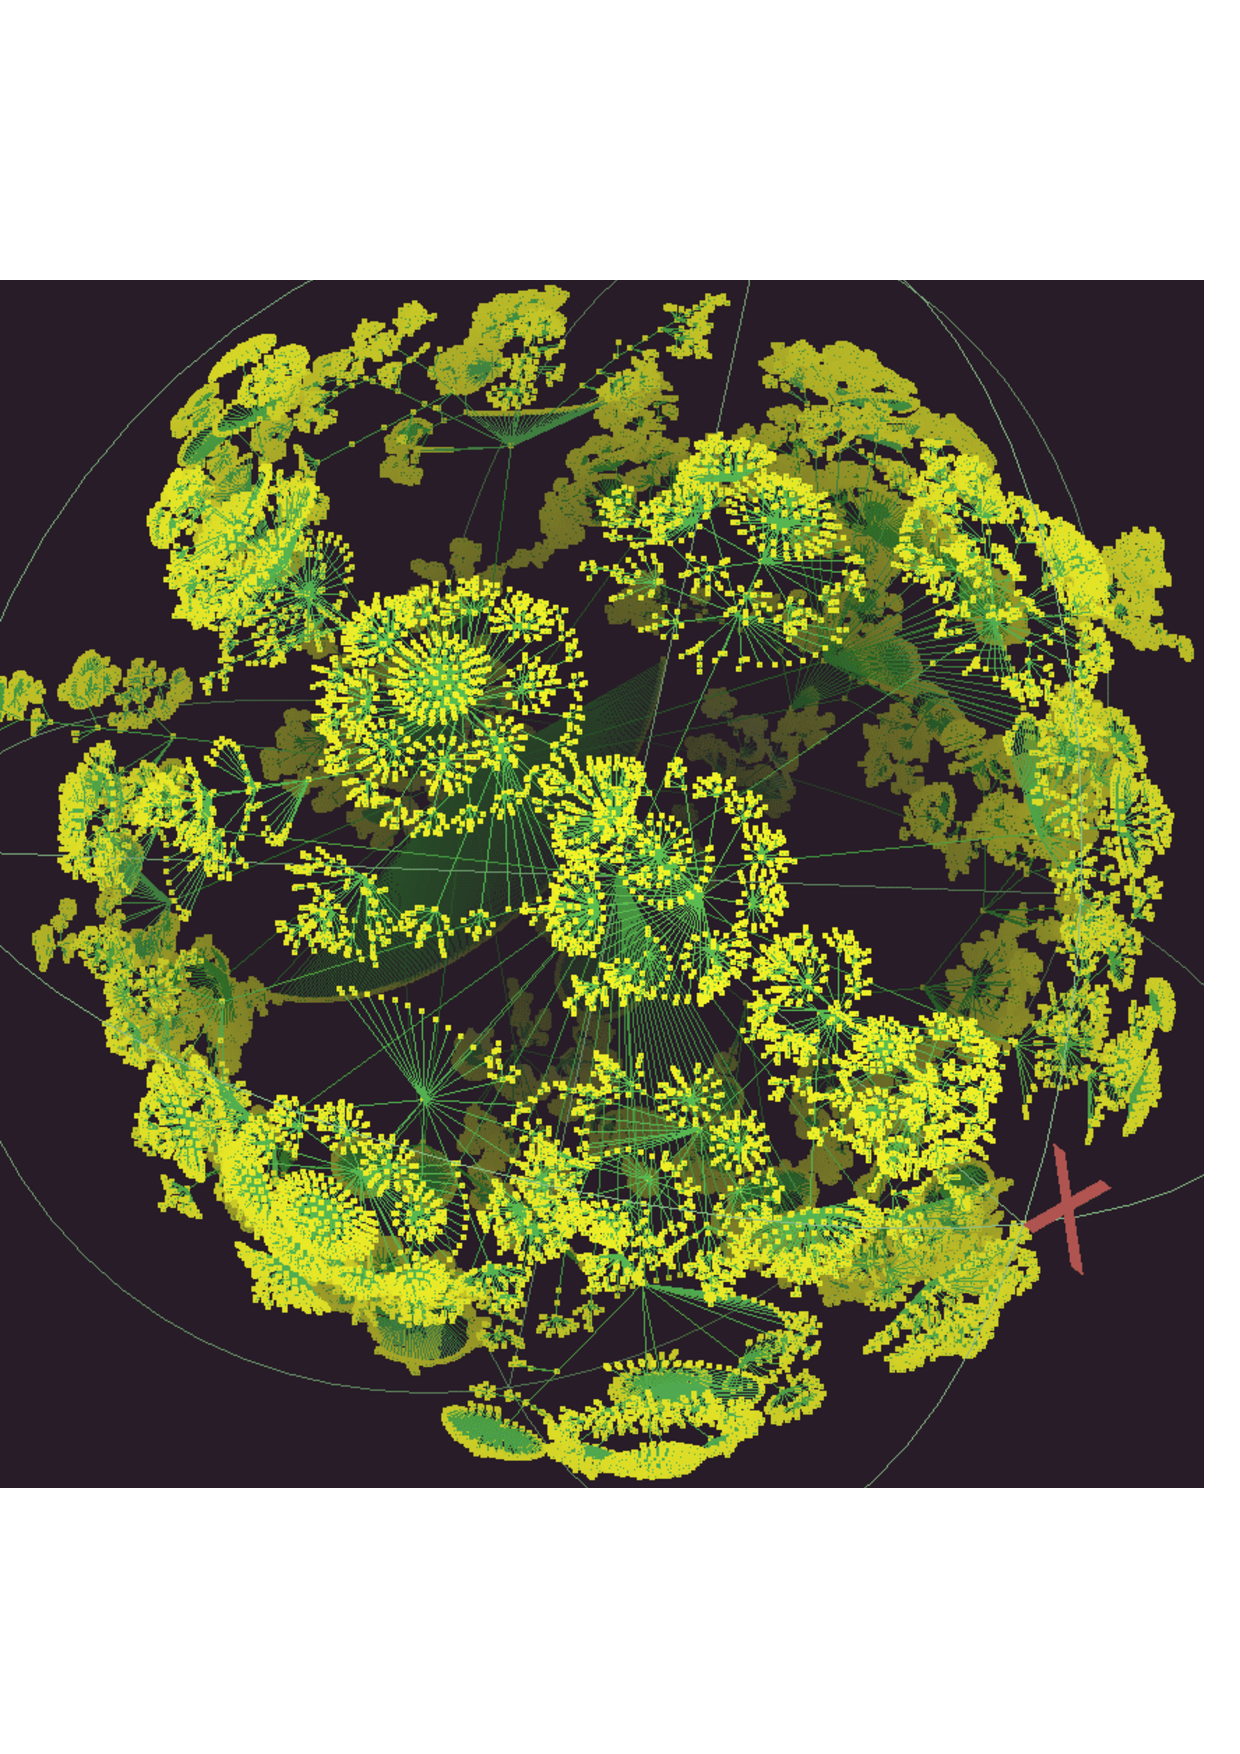
\includegraphics[width=0.481\textwidth]{webgraph_1}
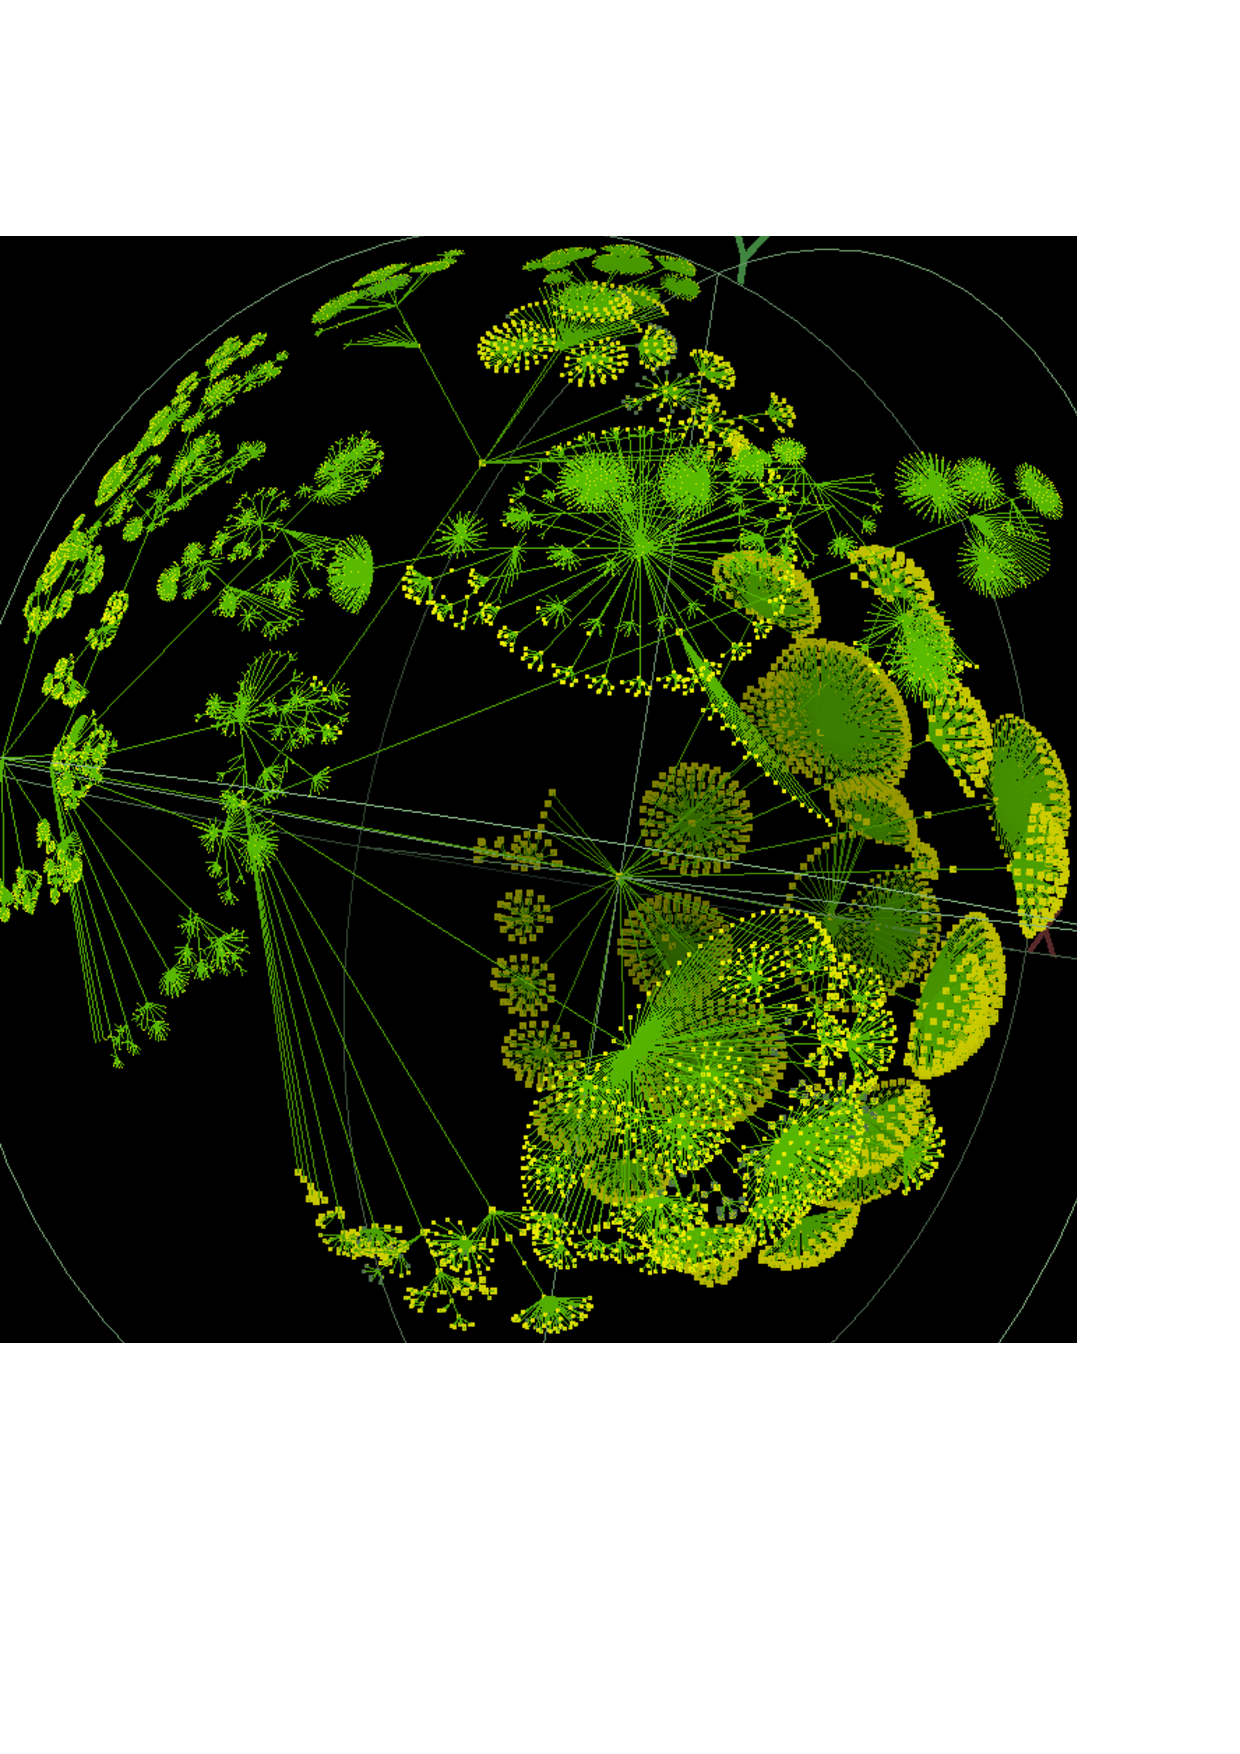
\includegraphics[width=0.47\textwidth]{webgraph_2}
\caption{Examples of real-world web-graphs of the internet, capturing their high-level random tree-like structure. Graphics attributed to the Center for Applied Internet Data Analysis (CAIDA), \texttt{\href{http://www.caida.org}{http://www.caida.org}}.} \label{fig:webgraph}
\end{figure*}

%
% Scale-Free Networks
%

\subsection{Scale-free networks}

\comment{To do}